% Template for FPL 2012 papers; to be used with:
%          spconf.sty   - ICASSP/ICIP LaTeX style file
%          IEEEtran.bst - IEEE bibliography style file

% Created:  Apr-May 2005 - Riku Uusikartano -- riku.uusikartano@tut.fi
% Modified: March-2012 - Daniel Mu�oz Arboleda -- damuz@unb.br
% --------------------------------------------------------------------------

\documentclass[10pt,a4paper]{article}

\usepackage{spconf,amsmath,epsfig}
\usepackage[brazilian]{babel} % Suporte para o Portugu�s
\usepackage[latin1]{inputenc} % Suporte para acentua��o sem necessidade dos comandos especiais.
%\usepackage[]{subfigure}
\usepackage[portuguese,algoruled,longend]{algorithm2e}
\usepackage{multirow}



% Titulo do documento
% -------------------
\title{Formato de Relat�rio de Laborat�rio de Sistemas Digitais 2}


% Nome dos autores
% ----------------
\name{
Fulano da Silva, Sutano Oliveira}
\address{Programa de Gradua��o em Engenharia Eletr�nica, Faculdade Gama\\
Universidade de Bras�lia\\
Gama, DF, Brasil\\
email: emailfulano@unb.br, emailsutano@unb.br}


\hyphenation{Tam-pe-re ela-bo-ra-cao}

\begin{document}

\maketitle

\begin{resumo}
Meu deus do ceu
\end{resumo}
\section{Introducao}
testando o atom

\section{Experimento}
Neste item descreva os procedimentos. Descreva o que deve ser feito com todos os detalhes como equipamentos e material utilizado. Procure ser detalhista na descri��o, de modo que qualquer pessoa que leia o seu relat�rio compreenda o que foi feito \cite{Cijvat2002}, \cite{Considine1983}. Aqui se descreve a sequ�ncia de etapas que foi realizada para que o experimento tivesse sucesso. Nesta se��o tamb�m s�o apresentados os desenvolvimentos te�ricos, que d�o suporte ao experimento assim como as estrat�gias experimentais empregadas. Conforme a complexidade do experimento, deve-se dividir esta se��o em sub-se��es \cite{Bellanger1976}.

\subsection{Tamanho do Relat�rio}
O trabalho completo, incluindo figuras e tabelas, deve ser limitado a 05 (cinco) p�ginas em tamanho A4 (21 cm x 29,7 cm). Por favor atenda a esta limita��o escrevendo de forma concisa e n�o reduzindo figuras e tabelas a tamanhos que sacrifiquem o entendimento dos s�mbolos e legendas nelas inclu�dos.

\subsection{Equa��es}
Todas as equa��es devem estar numeradas, colocando o n�-mero da equa��o entre par�nteses e alinhado � direita. A equa��o deve estar centralizada na coluna e verticalmente separada do texto por uma linha de texto (isto � autom�tico no formato \LaTeX de confer�ncias da IEEE).

\begin{equation}\label{eq1}
  H(z) = \frac{z^{-N}(1-z^{-R})^{N}}{(1-z^{-1})^{N}},
\end{equation}

onde ${N}$ and ${R}$ s�o algumas vari�veis, em formato tipo $italico$ tanto na equa��o como no texto.

O seguinte exemplo apresenta como representar conjuntos de equa��es relacionadas. Quando a equa��o requer usar duas colunas, o posicionamento correto � no topo da p�gina (vide equa��o \ref{eq3}). No caso de equa��es usando as duas colunas, o n�mero da equa��o est� verticalmente centralizado na equa��o.

% Exemplo de equa��es multiplas.
% ------------------------------
\begin{subequations}\begin{align}
  \label{eq2a} y(n)& = x(n-1) + a(n-1)\\
  \label{eq2b} a(n-1)& = x(n-2) + b(n-2)\\
  \label{eq2c}\begin{split}
  b(n)& = x(n-2) + a(n-2) + 1\\
  & = y(n-1) + 1.\end{split}
\end{align}\end{subequations}


% Exemplo de equa��o ocupando as duas colunas
% -------------------------------------------
\begin{figure*}[t]
\begin{equation}\label{eq3}
f_{h,\varepsilon}(x,y)= \int L_{x,z}\varphi(x)\rho_x(dz)+\biggl[\biggl(\int_0^{t_\varepsilon}L_{x,y^x(s)}\varphi(x)\,ds
  \biggr)+(\int_0^{t_\varepsilon}L_{x,y^x(s)}
    \varphi(x)\,ds -\mathbf{E}_{x,y}\int_0^{t_\varepsilon} L_{x,y_\varepsilon(\varepsilon s)}\varphi(x)\,ds\biggr)\biggr]
\end{equation}%
\end{figure*}

\subsection{Figuras e Tabelas}
Todas as figuras e tabelas devem estar numeradas. Texto e s�mbolos nelas inclu�dos devem ser de f�cil leitura, devendo-se evitar o uso de s�mbolos pequenos. Solicita-se a inclus�o de ilustra��es e/ou fotos de boa qualidade. Figuras, tabelas e suas legendas dever�o estar centradas no texto. Posicione a legenda abaixo da figura. Posicione o t�tulo de uma tabela acima da mesma. Um exemplo de figura � mostrado na Fig. \ref{fig1}.

\begin{figure}[htbp]
	\centering
		\includegraphics[scale=0.9]{Figuras/fig1_RNG.pdf}
		%\includegraphics[scale=0.9]{figures/fig1_RNG.eps}
	\caption{Gerador de n�meros aleat�rios em ponto flutuante}
	\label{fig1}
\end{figure}

Tabelas podem ser constru�das usando os comandos do \LaTeX. Um exemplo de tabela � mostrado na Tabela \ref{tab1}.

\begin{table}[t]
\caption{Exemplo de tabela.}\label{tab1}

\begin{minipage}[b]{1.0\linewidth}\centering
\renewcommand{\arraystretch}{1.2}
\begin{center}
\begin{tabular}{l|c|c}
\hline
 & Proposed design & Reference design
\\\hline\hline
 Data 1 & 1.12 mm$^2$ & 1.91 mm$^2$\\
\hline
 Data 2 & 32412 & 54213\\
\hline
  \hspace{-6pt}\begin{tabular}{l}Data 3\\[-5pt] (measured) \end{tabular}  & 8.2 mW & 11.3 mW\\
\hline
 Data 4 & \multicolumn{2}{c}{\begin{tabular}{c}some common properties\\[-5pt] for both designs \end{tabular}}\\
\hline
\end{tabular}
\end{center}
\end{minipage}
\end{table}

Denomine os eixos coordenados em gr�ficos, incluindo as respectivas unidades, sempre que aplic�vel. Da mesma forma, denomine colunas/linhas em tabelas, com respectivas unidades.


\section{Resultados}
Os resultados devem ser apresentados numa sequ�ncia que os correlacione com o experimento descrito na se��o anterior. Neste item os integrantes do grupo mostram os resultados em forma de tabela, gr�ficos, ou de acordo com a necessidade. Aqui tamb�m deve ser feita uma an�lise sobre cada um desses resultados. A forma das curvas, o valor lido nos instrumentos, etc. Nunca deixe um gr�fico ou uma tabela sem a devida interpreta��o! Um erro comum � colocar 2 ou mais gr�ficos e n�o especificar os porqu�s do que foi medido. Caso voc� perceba que algo aconteceu em laborat�rio que n�o est� de acordo com a teoria procure avaliar as raz�es.


\section{Discuss�o e Conclus�es}
Jamais esque�a este item! Neste item, descreva resumidamente os resultados observados e os seus significados. Exemplo: Com o aumento da frequ�ncia, observou-se que a tens�o de sa�da foi caindo. Isto aconteceu porque trata-se de um filtro passa baixas, o qual apresenta esta caracter�stica. Neste item os integrantes do grupo discutem o porqu� dos resultados obtidos, buscando demonstrar que eles atendem ao que foi solicitado e comprovam o sucesso do experimento.
Compara��es com valores obtidos por outros, em artigos, manuais ou \emph{data-sheets}, bem como sua compara��o com o que � esperado teoricamente, ajudam a comprovar o sucesso do experimento \cite{Henker1999}, \cite{Voit2010}.


\small
% IEEEtran is a LaTeX style file defining the reference formatting.
% -----------------------------------------------------------------
\bibliographystyle{IEEEtran}
\bibliography{IEEEabrv,labrefs}
%\bibliography{IEEEabrv,fpl_refs}


\end{document}